\documentclass{article}

\usepackage[margin=1in]{geometry}
\usepackage{amsmath}
\usepackage{graphicx}  % needed for figures

\title{Formalizing the ATM problem}
\author{Bryan O'Gorman, Tobias Stollenwerk}
\date{\today}

\begin{document}
\maketitle

These notes attempt to formalize the ATM problem: given a set of flights, schedule them in a way that minimizes cost.

\section{Configuration space}

At the highest level, the configuration space is a set of 4D trajectories, one for each flight.
Even with relatively coarsely discretized spacetime, that space is infeasably large.
Therefore we parameterize each trajectory by its deviations from the ideal, conflict-ignorant one.
Such deviations are of two types: temporal and spatial. 
A temporal deviation is simply a delayed start (typically on the order of up to 30 minutes). 
We assume that within the time-scale of such delays, the ideal conflict-ignorant trajectory is time-independent.
There are two types of spatial deviations: global and local.
A global spatial deviation changes the entire trajectory.
For example, one parameterization of global spatial deviations treats each trajectory as an arc in a plane perpendicular to the ground and considers smooth one-parameter curves to the projection of the trajectory onto the ground.
A local deviation consists of a set of maneuvers that change relatively small parts of the spatial trajectory.
Such maneuvers may introduce a delay, but, as with the delays due to temporal deviations, we assume that the subsequent trajectory is unaffected other than simply being delayed.

Henceforth, we focus on origination delays (temporal deviations) and maneuvers (local spatial deviations).

\section{Cost function}

In reality, the cost function results from factors such as fuel, labor, time, etc.; here we treat it as a unitless quantity that appropriately weights these factors.
Because we are interested in the relative costs of different configurations, we treat the cost of the configuration in which all flights are routed along their independently optimal trajectories, ignoring conflicts, and are exactly on time, as zero.
We further assume that the total cost is the sum of two different types of costs:
\begin{itemize}
  \item for each flight $i$, the cost $c_i^{\mathrm{late}}$ of being late on arrival,
  \item for every conflict $k$, the cost $c_k^{\mathrm{avoid}}$ of avoiding it.
\end{itemize}
The total cost therefore is 
\begin{equation*}
c = 
\sum_i c^{\mathrm{late}}_i + 
\sum_{k} c^{\mathrm{avoid}}_k
,
\end{equation*}
where each contribution to the cost function depends (implicitly as written so far) on the configuration space.
%Here we treat each conflict as between two flights. 
%If three flights were to conflict in the same neighborhood of spacetime, then there would be three individual conflicts to consider, though the actions to take and costs of doing so would be interdependent.
Because the lateness and avoidance costs are associated with flights and conflicts, respectively, we write simply $c_i = c_i^{\mathrm{late}}$ and $c_{k} = c_{k}^{\mathrm{avoid}}$ where the distinction is clear from context.
%For notational convenience, all conflicts, regardless of the flights involved, are indexed by a single, time-ordered $k$, in which case many of the $c_{ijk}$ are trivially zero (i.e. when flights $i$ and $j$ are not involved or potentially involved in conflict $k$).
Henceforth, we simplify things by ignoring the direct cost of the local maneuvers. 
However, they will still indirectly contribute to the cost function via their introduction of further delays.
The quantity to minimized can then be written
\begin{equation*}
c = 
\sum_i c_i (D_i),
\end{equation*}
where $D_i = d_i + \sum_k d_{ik}$ is the delay of flight $i$ at its destination, which will be a function of its origination delay $d_i$ and delays $\{d_{ik}\}$ introduced by local maneuvers.
%As for $c_{ijk}$ we define $d_{ik}$ for every flight $i$ and every conflict $k$, but many of them will be trivially zero (i.e. when flight $i$ is not involved or potentially involved in conflict $k$).
For notational simplicity we define $d_{ik}$ for every flight $i$ and every conflict $k$, but many of them will be trivially zero (i.e. when flight $i$ is not involved or potentially involved in conflict $k$).

Lastly, we simplify things further by assuming that all destination delays are equally important, (which comes by necessity from the absence of information to the contrary), so that the quantity to minimize is simply the total delay of all flights:\footnote{The lack of information with respect to the relative importance of flights in reality only requires that all $c_i$ be the same function. One could imagine minimizing the $L_2$ norm(which would help avoid having a few very late flights) rather than the $L_1$ norm as we do here, or indeed any other function. The simple sum here is the one currently used by Olga et al., and has the advantage of being most conducive to mapping to QUBO.}
\begin{equation*}
c = D = \sum_i D_i.
\end{equation*}

\section{Classical subroutines}
We further assume the availability of the following two subroutines, whose resource requirements we regard as negligible:
\begin{itemize}
\item given a flight (its origin and destination, and properties of the plane), return the optimal route
\item given two flight paths, return the set of conflicts
\item given two flight paths and start times, and one of the conflicts from above, return the ``delay frontier'' in the sparse case (described below) or the set of possible conflict-avoiding maneuvers in general
\end{itemize}

\section{Assumptions made}
\begin{itemize}
\item For each flight, the optimal route is time-independent (both spatially and in duration) over the timescale of possible delays.
For example, if the flight has no potential collisions, its lateness on arrival will exactly equal its departure delay.
\item Actively avoiding a collision (rather than avoiding via departure delays) does not change the cost of actively avoiding other collions on the same flight path. In reality, one could reason, e.g. that the little bit of fuel used in each active collision avoidance could add up to a disastrously empty tank, but in general we would like the effect of active collision avoidances to be as litle as possible.
Similarly, one could argue that the plane burns fuel while idling.
\end{itemize}

\section{Potentially helpful assumptions}
\begin{itemize}
\item All conflicts are pairwise. That is, when two planes have a potential conflict, there are no other planes nearby. 
Furthermore, when this conflict is avoided, it does not create a conflict with another flight. 
(This may be the most unreasonable assumption, e.g. near major airports or on crowded jetstreams.)
\item Collisions are symmetric. That is, the cost of avoiding them is a function only of the magnitude of the difference in delays of the two flights up until that point. For example, the cost of avoiding a collision between $i$ and $j$ is the same whether $i$ is delayed by $d$ or $j$ is.
\item The lateness cost functions are non-decreasing; we might as well allow it to be negative for earliness, though that could be compiled away by pushing the range of available departure times earlier. This is obviously satisfied for the linear cost functions with unit slope used here, and hard to imagine relaxing.
\end{itemize}

\section[Towards a solution] {Towards a solution\footnote{
It remains to be proven that this problem is hard, either in general or for realistic values of its parameters, e.g. cost functions.}}

Let $D_{ik} = d_i + \sum_{k' < k} d_{ik}$ be the delay of flight $i$ when it reaches potential conflict $k$, and $a_k$ be some parameterization of the maneuvers chosen for conflict $k$.
Then the general cost function is, with all dependencies explicit,
\begin{equation*}
D(\mathbf d, \mathbf a) = \sum_i D_i(\mathbf d, \mathbf a)
= 
\sum_i \left(d_i + \sum_k d_{ik} (\mathbf D_{k}, \mathbf a_k)\right),
\end{equation*}
where $\mathbf d = (d_i)_{i=1}^n$ and $\mathbf a = (a_k)_{k=1}^m$ represent all the origination delays and maneuver parameters, respectively; $\mathbf D_k = (D_{ik})_{i \in I_k}$, where $I_k$ is the set of flights involved or potentially involved in conflict $k$; and $\mathbf a_k = (a_{k'})_{k'=1}^{k-1}$.
This is the most general cost function we can write down using local maneuvers and the assumptions made in previous work by Olga et al.

\subsection{Sparse case}

First, we describe a method for solving the ``sparse'' version of the problem. 
By sparsity, we mean that all conflicts are between only two trajectories and that no other trajectories are nearby in spacetime, so that potential maneuvers for avoiding a conflict between two flights do not introduce additional conflicts with other flights.\footnote{This could be extended to an $m$-sparse version, where each conflict can affect $m-1$ others.}

The delays $(d_{ik}, d_{jk})$ introduced by maneuvering to avoid conflict $k$ between flights $i$ and $j$ are solely a function of the delays $(D_{ik}, D_{jk})$ of those flights up until the conflict and the maneuver $a_{k}$ chosen to avoid the conflict.
In particular, the delay depends only on the difference of the delays $\Delta_{k} = D_{ik} - D_{jk}$ (where the $i$ and $j$ for a given $k$ are implictly specified and have a canonical ordering).
It's plausible to assume that it furthermore depends only on the magnitude of this difference $|D_{ik} - D_{jk}|$, though it's not yet clear that that will help.

In general, the avoidance delays as a function of this difference $\Delta_{k}$ will be a function of the specific maneuvers chosen. 
For a given $\Delta_{k}$ that there is a minimal delay of each flight $d_{ik}^*$ assuming that the other is unchanged, and there is (presumably) a concave ``delay frontier'' in the region $[0, d_{ik}^*] \times [0, d_{jk}^*]$ connecting $(d_{ik}^*, 0)$ and $(0, d_{jk}^*)$ that gives the possible delays $(d_{ik}, d_{jk})$. 
We parameterize this curve by $a_{k} \in [0, 1]$.
More generally, there is a ``delay surface'' when various values of $\Delta_{k}$ are considered.

The most general cost function in the sparse case is 
\begin{equation*}
D(\mathbf d, \mathbf a) 
=
\sum_i \left(d_i + \sum_k d_{ik} (D_{ik} - D_{jk}, a_k)\right).
\end{equation*}

In the (overly simplistic) case where maneuvers do not introduce any further delays, we have simply
\begin{equation*}
D = 
\sum_i
\left(d_i + \sum_k d_{ik}(d_i - d_j) \right),
\end{equation*}
where
\begin{equation*}
    d_{ik} = \begin{cases} 0, & \text{collision $k$ can be avoided given delays $d_i$ and $d_j$},\\
    \infty, & \text{otherwise}.
\end{cases}
\end{equation*}
For the assumption that maneuvers do not introduce further delays to make any sense at all, we must bound their size, which is why some conflicts simply cannot be avoided within this approximation.
Of course, we define $d_{ik}$ as piece-wise infinite for consistency with the rest of these notes, but in practice this would be implemented as a hard constraint.
(Interestingly, this notational device has the morose interpretation that if the flights do collide, the further delay introduced is indeed infinite.)

Both of the above forms invite straightforward QUBO formulations.
Discretize and introduce bits for each discrete value for the variables $d_i$, $d_{ik}$, $\Delta_k = D_{ik} - D_{jk}$, and $a_k$:
\begin{equation*}
    C = D + x C^{\mathrm{one}} + y C^{\mathrm{equal}},
\end{equation*}
where 
\begin{equation*}
D = 
\sum_{i} \sum_{\alpha} \alpha d_{i\alpha}
+
\sum_{ik} \sum_{\beta} \beta d_{ik\beta}
\end{equation*}
is the delay to be minimized,
\begin{equation*}
C^{\mathrm{one}}
=
\sum_i \left(\sum_{\alpha} d_{i\alpha}- 1 \right)^2 
+
\sum_{ik} \left(\sum_{\beta} d_{ik\beta} - 1\right)^2
+
\sum_{ik} \left(\sum_{\gamma} \Delta_{ik\gamma} - 1\right)^2
+
\sum_{k} \left(\sum_{\delta} a_{k\delta}- 1\right)^2
\end{equation*}
is the penalty function ensuring that each variable has a well defined value encoded by a single bit,
\begin{align*}
C^{\mathrm{equal}}
&=
\sum_{k} \left[
\left(\sum_{\alpha} d_{i\alpha} + \sum_{k' < k} \sum_{\beta} \beta d_{ik\beta}\right)
-
\left(\sum_{\alpha} d_{j\alpha} + \sum_{k' < k} \sum_{\beta} \beta d_{jk\beta}\right)
-
\left(\sum_{\gamma} \gamma \Delta_{k\gamma}\right)\right]^2
+ \\
&\hphantom{=,}
\sum_{ik} \left[
    \left(\sum_{\beta} \beta d_{ik\beta}\right) - 
\left(\sum_{\gamma \delta} d_{ik} (\gamma, \delta) \gamma_{k\gamma} a_{k\delta}\right)\right]^2
\end{align*}
is the penalty function ensuring that $\Delta_k = D_{ik} - D_{jk}$ and $d_{ik} = d_{ik}(\Delta_k, a_k)$, 
the Greek indices represent the discrete values that the corresponding quantities can assume, and $x$ and $y$ are penalty weights.\footnote{In practice we could have varying penalty weights for the various penalties.}

We could make a further approximation and for each conflict pick some optimal-in-expectation $a_k$, thereby removing that variable from the formulation.
We could also suitably parameterize the ``delay surface'' so that the cost function could be written in a functional form.

\subsection{Dense case}
The sparsity condition assumed above is in general false, even when ignoring near-airport trajectories.
The other extreme is the ``dense'' case, in which all flights are restricted to a ``highway'' as in Olga's thesis.
An appropriate QUBO for that problem is relatively straightforward, and can be written explicitly if needed.

\subsection{General case}
General instances fall into neither of the above extremes.
One potential solution is to use some sort of master-slave subproblem decomposition to combine solvers for each extremal case into a general solution.

\section{Conflict calculation}
The flights are indexed by
\begin{equation*}
    i \in \{i, \dots, n\}
\end{equation*}
For each flight $i$, the wind-optimal trajectories are given as a sequence of 4-dimensional space-time points
\begin{equation*}
    \tau_i = \{p^i_1, \dots, p^i_{M_i}\}
\end{equation*}
with
\begin{equation*}
    p^i_j = (\mathbf{r}^i_j, t^i_j \Delta_t) = \left( \underbrace{x^i_j \Delta_\text{lat}, y^i_j \Delta_\text{lon}, z^i_j \Delta_v}_{=:\mathbf{r}^i_j}, t^i_j \Delta_t\right)
\end{equation*}
The sequence of points in space are given by
\begin{equation*}
    r_i = \{\mathbf{r}^i_1, \dots, \mathbf{r}^i_{M_i}\}
\end{equation*}
Conflicts may occur if multiple flight trajectories
\begin{equation*}
    \{\tau_i : i \in I \subseteq \{1, \dots, n\}\}
\end{equation*}
become to close to each other in time and space.
In the following, we will reduce the multiple flights involved in a given conflict to pairwise conflicts.
With this, a conflict always involves only two flights.

\subsection{Potential conflicts}
Given the trajectories we can calculate all the spatial conflicts.
The existence of a real conflict depends on the arrival time of both flights $i$ and $j$ at the spatial conflict $k$, $T_{ik}$ and $T_{jk}$ (see figure~\ref{fig:spatial_conflicts}). 
The corresponding departure times from the spatial conflict are denoted by 
\begin{equation*}
    T'_{ik} = \frac{L_k}{v_i} + T_{ik}
\end{equation*}
where $L_k$ spatial length of the spatial conflict $k$ and $v_i$ is the constant velocity of flight $i$.
\begin{figure}[htpb]
    \centering
    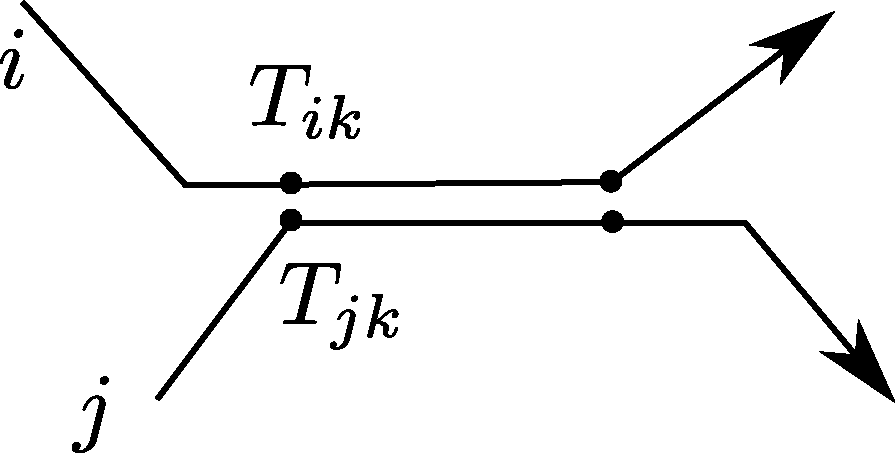
\includegraphics[width=0.3\linewidth]{pics/spatial_conflict_parallel.pdf}
    \hspace{1cm}
    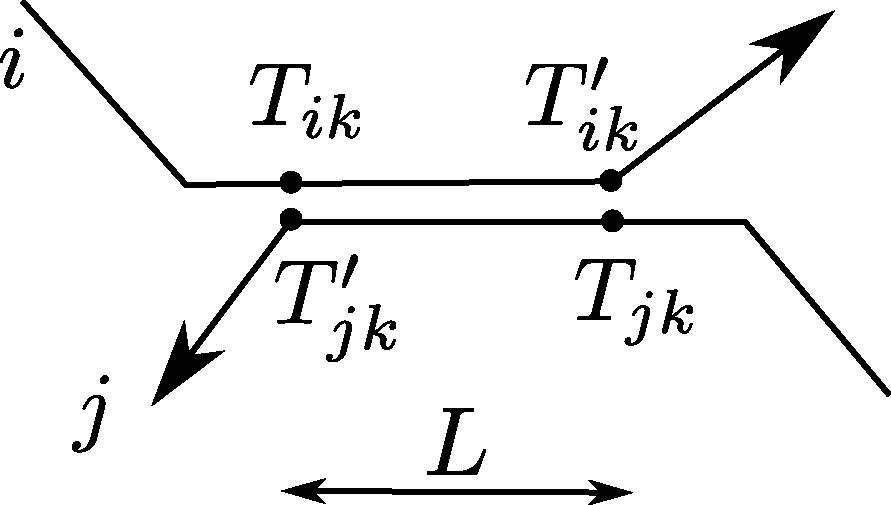
\includegraphics[width=0.3\linewidth]{pics/spatial_conflict_anti_parallel.pdf}
    \caption{Parallel and antiparallel spatial conflict}
    \label{fig:spatial_conflicts}
\end{figure}

\begin{itemize}
    \item {\bf Parallel conflict:}
        A real conflict exists if the difference between the arrival times is smaller than a threshold $\Delta_p$ which depends on the trajectories, in particular the speed and position of both flights.
        \begin{equation*}
            \bigl| \underbrace{T_{jk} - T_{ik}}_{\Delta_k} \bigr| < \Delta_p
        \end{equation*}
        with
        \begin{equation*}
            \Delta_p = \Delta_p(v_i, v_j, r_i, r_j)
        \end{equation*}
        This can also be written as
        \begin{equation}  \label{eqn:conflict_parallel}
            -\Delta_p < \Delta_k < \Delta_p 
        \end{equation}
        
    \item {\bf Antiparallel conflict:}
        A real conflict exists if 
        \begin{equation*}
            T'_{ik} - T_{jk} < \Delta^1_{ap}(v_i, v_j, r_i, r_j)
        \end{equation*}
        and
        \begin{equation*}
            T'_{jk} - T_{ik} < \Delta^2_{ap}(v_i, v_j, r_i, r_j)
        \end{equation*}
        Hence
        \begin{eqnarray*}
            \frac{L_k}{v_i} + \underbrace{T_{ik} - T_{jk}}_{-\Delta_k} < \Delta^1_{ap} \\
            \frac{L_k}{v_j} + \underbrace{T_{jk} - T_{ik}}_{\Delta_k} < \Delta^1_{ap} 
        \end{eqnarray*}
        This yields
        \begin{equation} \label{eqn:conflict_antiparallel}
            \frac{L_k}{v_i} - \Delta^1_{ap} < \Delta_k < \Delta^2_{ap} - \frac{L_k}{v_j}
        \end{equation}
\end{itemize}

Now, we introduce the notion of a \textit{potential} conflict.
The arrival time $T_{ik}$ is given by the arrival time in the wind optimal case $t_{ik}$ plus the delay it picked up due to earlier conflict avoiding maneuvers or a departure delay $D_{ik}$. 
\begin{equation*}
    T_{ik} = t_{ik} + D_{ik} \quad \forall i, k
\end{equation*}
and the difference of the arrival time of the two flights $i$ and $j$ at spatial conflict $k$ is given by
\begin{eqnarray*}
    \Delta_k &=& T_{ik} - T_{jk} \\
             &=& t_{ik} - t_{jk} + D_{ik} - D_{jk}
\end{eqnarray*}
The maximal value of $D_{ik}$, $\forall i, k$ is bounded from above by some $D^{\text{max}}$.
Hence, $\Delta_k$ is bounded by
\begin{equation} \label{eqn:potential_conflict}
    (t_{ik} - t_{jk} - D^{\text{max}})< \; \Delta_k \; < (t_{ik} - t_{jk} + D^{\text{max}})
\end{equation}
Therefore, we identify a spatial conflict $k$ as a \textbf{potential conflict} if for a $\Delta_k$ which is bounded by \eqref{eqn:potential_conflict}, one of the inequalities \eqref{eqn:conflict_parallel} or \eqref{eqn:conflict_antiparallel} is fulfilled.

From now on, all indices $k$ will denote potential conflicts.

\subsection{Calculation of the conflict arrival times}
A classical precalculation gives us all potential conflicts $k$, and therefore a mapping
\begin{equation*}
    k \mapsto \{i, j\} = I_k
\end{equation*}
We can get the potential conflicts in which the flight $i$ is involved, ordered by their temporal appearance:
\begin{equation*}
    i \mapsto (k^i_1, \dots, k^i_{N_i})
\end{equation*}
A conflict avoiding maneuver delays the flight by a certain amount of time
\begin{equation*}
    d_{ik} \quad, \quad  k\in\{k^i_1, \dots, k^i_{N_i}\}
\end{equation*}
The departure delays $d_i$ can be seen as the result of a conflict $k^i_0$ at departure which only involved the flight itself.
\begin{equation*}
    d_i \to d_{ik^i_0}
\end{equation*}
Therefore we have
\begin{equation*}
    d_{ik} \quad, \quad  k\in\{k^i_0, k^i_1, \dots, k^i_{N_i}\}
\end{equation*}
The arrival time of flight $i$ at conflict $k$ then reads
\begin{equation*}
    T_{ik} = t_{ik} + \sum_{p \in K^<_{ik}} d_{ip}
\end{equation*}
where the set of conflicts the flight $i$ was involved in before $k$ is given by
\begin{equation*}
    K^<_{ik} = \{\tilde k : \tilde k \in\{k^i_0, \dots, k^i_{N_i}\}, \tilde k < k\}
\end{equation*}
and $t_{ik}$ denotes the arrival time of flight $i$ at a potential conflict $k$ in the absence of any delays, i.e.\ in the wind-optimal case.

\section{Models}
\subsection{Independent delay model}
We assume, that the delays $d_{ik}$ are independent of each other. 
This means at every conflict $k \in  \{k^i_0, \dots, k^i_{N_i}\}$ for a given flight $i$, we can introduce a delay $d_{ik}$ which is independent of the delays of the other flight $d_{jk}$ for $j\neq i$ involved in the potential conflict.
This is in contrast to Bryan's model which couples both delays thought a \textit{delay frontier}.
Our goal is to write down a cost function which penalizes the total delay as well as the appearance of real conflicts (depending on the arrival times).

The variables we try to optimize are the delays $d_{ik}$.
We bound and discretize the values they can assume by introducing binary variables $d_{ik\beta}\in\{0, 1\}$ :
\begin{equation*}
    d_{ik} = \Delta_d \sum_\beta \beta d_{ik\beta}
\end{equation*}
The total delay is given by
\begin{equation} \label{eqn:idm_cost_delay}
    D(\{d_{ik}\}) = \Delta_d \sum_k \sum_{i \in I_k} \sum_\beta \beta d_{ik\beta}
\end{equation}
The term which ensures the uniqueness of the variables $d_{ik}$ reads
\begin{equation} \label{eqn:idm_cost_delay_unique}
    D^\text{one}(\{d_{ik}\})  =  \sum_k \sum_{i \in I_k} \left( \sum_\beta d_{ik\beta} - 1\right)^2
\end{equation}
In order to penalize the a real conflict, we need to write down the difference in the conflict arrival times in terms of the binary variables.
\begin{eqnarray}
    \Delta_k &=& T_{ik} - T_{jk} \notag \\
             &=& t_{ik} - t_{jk} + \Delta_d \left( \sum_\beta \sum_{p\in K^<_{ik}} \beta d_{ip\beta}  - \sum_\gamma \sum_{q\in K^<_{jk}} \gamma d_{jq\gamma} \right) \label{eqn:idm_delay_difference}
\end{eqnarray}
%With \eqref{eqn:conflict_parallel} we have a real conflict in the parallel case if
%\begin{equation*}
    %\Delta_k \in [-\Delta_p, \Delta_p]
%\end{equation*}
%and in the antiparallel case \eqref{eqn:conflict_antiparallel} if
%\begin{equation*}
    %\Delta_k \in \left[\frac{L_k}{v_i} - \Delta^1_{ap}, \Delta^2_{ap} - \frac{L_k}{v_j}\right]
%\end{equation*}
According to \eqref{eqn:conflict_parallel}, \eqref{eqn:conflict_antiparallel} and \eqref{eqn:potential_conflict} a conflict is avoided if the following holds:
\begin{equation*} \label{eqn:idm_slack_greater_parallel}
    \Delta_p < \Delta_k < (t_{ik} - t_{jk} + D^{\text{max}})
\end{equation*}
or
\begin{equation*} \label{eqn:idm_slack_lesser_parallel}
     (t_{ik} - t_{jk} - D^{\text{max}}) < \Delta_k < -\Delta_p
\end{equation*}
for a parallel conflict, and
\begin{equation*} \label{eqn:idm_slack_greater_antiparallel}
    \Delta^2_{ap} - \frac{L_k}{v_j} < \Delta_k < (t_{ik} - t_{jk} + D^{\text{max}})
\end{equation*}
or
\begin{equation*} \label{eqn:idm_slack_lesser_antiparallel}
     (t_{ik} - t_{jk} - D^{\text{max}}) < \Delta_k < \frac{L_k}{v_i} - \Delta^1_{ap}
\end{equation*}
for an antiparallel conflict.
We introduce the following notation for covering both the above cases.
\begin{equation*} \label{eqn:idm_slack_greater}
    \Delta^+_\text{min} < \Delta_k < \Delta^+_\text{max}
\end{equation*}
\begin{equation*} \label{eqn:idm_slack_lesser}
    \Delta^-_\text{min} < \Delta_k < \Delta^-_\text{max}
\end{equation*}
With this, we can introduce two slack variables
\begin{equation} \label{eqn:idm_slack_greater}
    y^+_k =  \Delta_k - \Delta^+_\text{min} \in [0, \Delta^+_\text{max} - \Delta^+_\text{min}]
\end{equation}
\begin{equation} \label{eqn:idm_slack_lesser}
    y^-_k =  \Delta_k - \Delta^-_\text{min} \in [0, \Delta^-_\text{max} - \Delta^-_\text{min}]
\end{equation}
By writing these slack variables in terms of binary variables $y^\pm_{k\alpha}$, we get
\begin{equation} \label{eqn:idm_slack_binary}
    y^\pm_k = \Delta_{y\pm} \sum_\alpha \alpha y^\pm_{k\alpha}
\end{equation}
With \eqref{eqn:idm_delay_difference}, \eqref{eqn:idm_slack_lesser}, \eqref{eqn:idm_slack_greater} and \eqref{eqn:idm_slack_binary} the contributions to the cost function which ensures the above inequalities, reads
\begin{equation} \label{eqn:idm_cost_conflict}
    S(\{d_{ik}\})  = \sum_{\lambda \in \{+, -\}} \sum_{\substack{k\\i\in I_k}} \left( t_{ik} - t_{jk} + \Delta_d \left( \sum_\beta \sum_{p\in K^<_{ik}} \beta d_{ip\beta}  - \sum_\gamma \sum_{q\in K^<_{jk}} \gamma d_{jq\gamma} \right) - \Delta^\lambda_\text{min} - \Delta_{y\lambda} \sum_\alpha \alpha y^\lambda_{k\alpha} \right)^2
\end{equation}
The contribution ensuring the uniqueness of the slack variables reads
\begin{equation} \label{eqn:idm_cost_conflict_unique}
    S^\text{one}(\{d_{ik}\})  = \sum_{\lambda \in \{+, -\}} \sum_k \left( \sum_\alpha \alpha y^\lambda_{k\alpha} - 1 \right)^2
\end{equation}
The whole cost function is the sum of \eqref{eqn:idm_cost_delay}, \eqref{eqn:idm_cost_delay_unique}, \eqref{eqn:idm_cost_conflict} and \eqref{eqn:idm_cost_conflict_unique}
\begin{equation*}
    C_\text{IDM}(\{d_{ik}\})  = D(\{d_{ik}\}) + D^\text{one}(\{d_{ik}\}) + S(\{d_{ik}\}) + S^\text{one}(\{d_{ik}\})
\end{equation*}

\subsection{Delay Frontier Model}
This is a Bryan's model written down in more detail.
Here, the delays are the result of a conflict avoiding maneuver.
The delays of the involved flights are a function of the difference in arrival times $\Delta_k$ and a maneuver parameter $a_k$
\begin{equation} \label{eqn:dfm_delay_frontier}
    d_{lk} = d_l(\Delta_k, a_k) \quad l \in I_k
\end{equation}
where 
\begin{equation*}
    a_k = \Delta_a \sum_\beta \beta a_{k\beta} \in [0, 1]
\end{equation*}
and
\begin{equation*}
    \Delta_k = \tilde \Delta \sum_\alpha \alpha \Delta_{k\alpha} \quad \in [\Delta^\lambda_\text{min}, \Delta^\lambda_\text{max}], \quad \lambda \in \{+, -\}
\end{equation*}
The form of this function has to be determined.
After discretizing its arguments, we can write
\begin{equation*}
    d_{lk} = d_l(\alpha, \beta) \quad l \in I_k
\end{equation*}
Therefore, we only need to store the return values of the above function for the finite set of arguments, i.e.\ all combinations of $\alpha$ and $\beta$.
To ensure uniqueness, we add the cost function term
\begin{equation} \label{eqn:dfm_cost_maneuver_unique}
    C^\text{one}(\{d_{ik}\})  =  \sum_k \left( \sum_\beta a_{k\beta} - 1\right)^2 + \sum_k \left( \sum_\alpha \Delta_{k\alpha} - 1\right)^2
\end{equation}
In order for \eqref{eqn:dfm_delay_frontier} to be fulfilled for the optimal solution of the problem, we add the following term to the cost function
\begin{equation} \label{eqn:dfm_cost_delay_frontier}
    S^d(\{d_{ik}\})  = \sum_{\substack{k\\l\in I_k}} \left(\Delta_d \sum_\beta \beta d_{lk\beta} - \sum_{\alpha, \beta} d_l(\alpha, \beta) \Delta_{k\alpha} a_{k \beta}\right)^2
\end{equation}
In the same way, we make \eqref{eqn:idm_delay_difference} hold, by adding 
\begin{equation} \label{eqn:dfm_cost_delay_difference_relation}
    S^\Delta(\{d_{ik}\})  = \sum_{\substack{k\\ \{i, j\}\in I_k}} \left( t_{ik} - t_{jk} + \Delta_d \left( \sum_\beta \sum_{p\in K^<_{ik}} \beta d_{ip\beta}  - \sum_\gamma \sum_{q\in K^<_{jk}} \gamma d_{jq\gamma} \right) - \tilde \Delta \sum_{\alpha} \alpha \Delta_{k\alpha}\right)^2
\end{equation}
By combining \eqref{eqn:idm_cost_delay}, \eqref{eqn:idm_cost_delay_unique}, \eqref{eqn:dfm_cost_maneuver_unique}, \eqref{eqn:dfm_cost_delay_frontier} and \eqref{eqn:dfm_cost_delay_difference_relation}, the cost function for the delay frontier model reads
\begin{equation*}
    C_\text{DFM}(\{d_{ik}\})  = D(\{d_{ik}\}) + D^\text{one}(\{d_{ik}\}) + C^\text{one}(\{d_{ik}\}) + S^d(\{d_{ik}\}) + S^\Delta(\{d_{ik}\})
\end{equation*}
\subsubsection{Variations of the Delay frontier model}
We can reduce the number of variables by
\begin{enumerate}
    \item Both flights will always \textit{split the delay}: Set $a_k$ to a fixed value inside $[0, 1]$, presumably $a_k = 0.5$. This would eliminate all variables $a_{k\beta}$.
    \item One flight makes a detour, the other remains on the wind-optimal route: Reduce the possible values values of $a_k$ to either $0$ or $1$. Hence $a_k$ itself becomes a binary variable.
\end{enumerate}


\subsection{Reduction of variables}
Possible measures to reduce the number of variables in the above models
\begin{itemize}
    \item Use binary representation instead of unary representation for all variables
    \item Make the maximal delay dependent on the conflict $D^\text{max} \to D^\text{max}_k$ since the maximal delay will depend on the specifics of the conflict, like velocity and spatial path.
\end{itemize}

\end{document}
